\documentclass[10pt,twocolumn, nofootinbib]{revtex4-1}
%\documentclass[aps,pra,10pt,twocolumn,floatfix,nofootinbib]{revtex4-1}
%\documentclass[10pt,twocolumn,letterpaper]{article}

\usepackage{amsmath}
\usepackage{amsfonts}
\usepackage{graphicx}
\usepackage{enumitem}
\usepackage{hyperref}
\hypersetup{
	colorlinks=true,
	citecolor=blue,
	urlcolor=blue,
	linkcolor=blue
}
\urlstyle{same}
\frenchspacing


\begin{document}

\title{Assumptions of Physics overview: \\
	experimental verifiability and topology }
\author{Gabriele Carcassi, Christine A. Aidala}
\affiliation{Physics Department, University of Michigan, Ann Arbor, MI 48109}

\date{\today}


\begin{abstract}
We briefly show how the use of topological spaces and $\sigma$-algebras in physics can be rederived and understood as the fundamental requirement of experimental verifiability. A set of experimentally distinguishable objects will necessarily be endowed with a topology that is Kolmogorov (i.e. $T_0$) and second countable, which puts severe constrains on the space of well-formed scientific theories. These idea can be taken as a first step in a general mathematical theory for experimental science. This work is an overview of some of the results of Assumptions of Physics, a project that aims to identify a handful of physical principles from which the basic laws can be rigorously derived  (\url{https://assumptionsofphysics.org}).
\end{abstract}

\maketitle

\section{Introduction}

The overall structure (see \cite{AoPBook} for more details) can be summed up in the following diagram that can be used as a guide throughout this note.

\begin{figure}[h]
	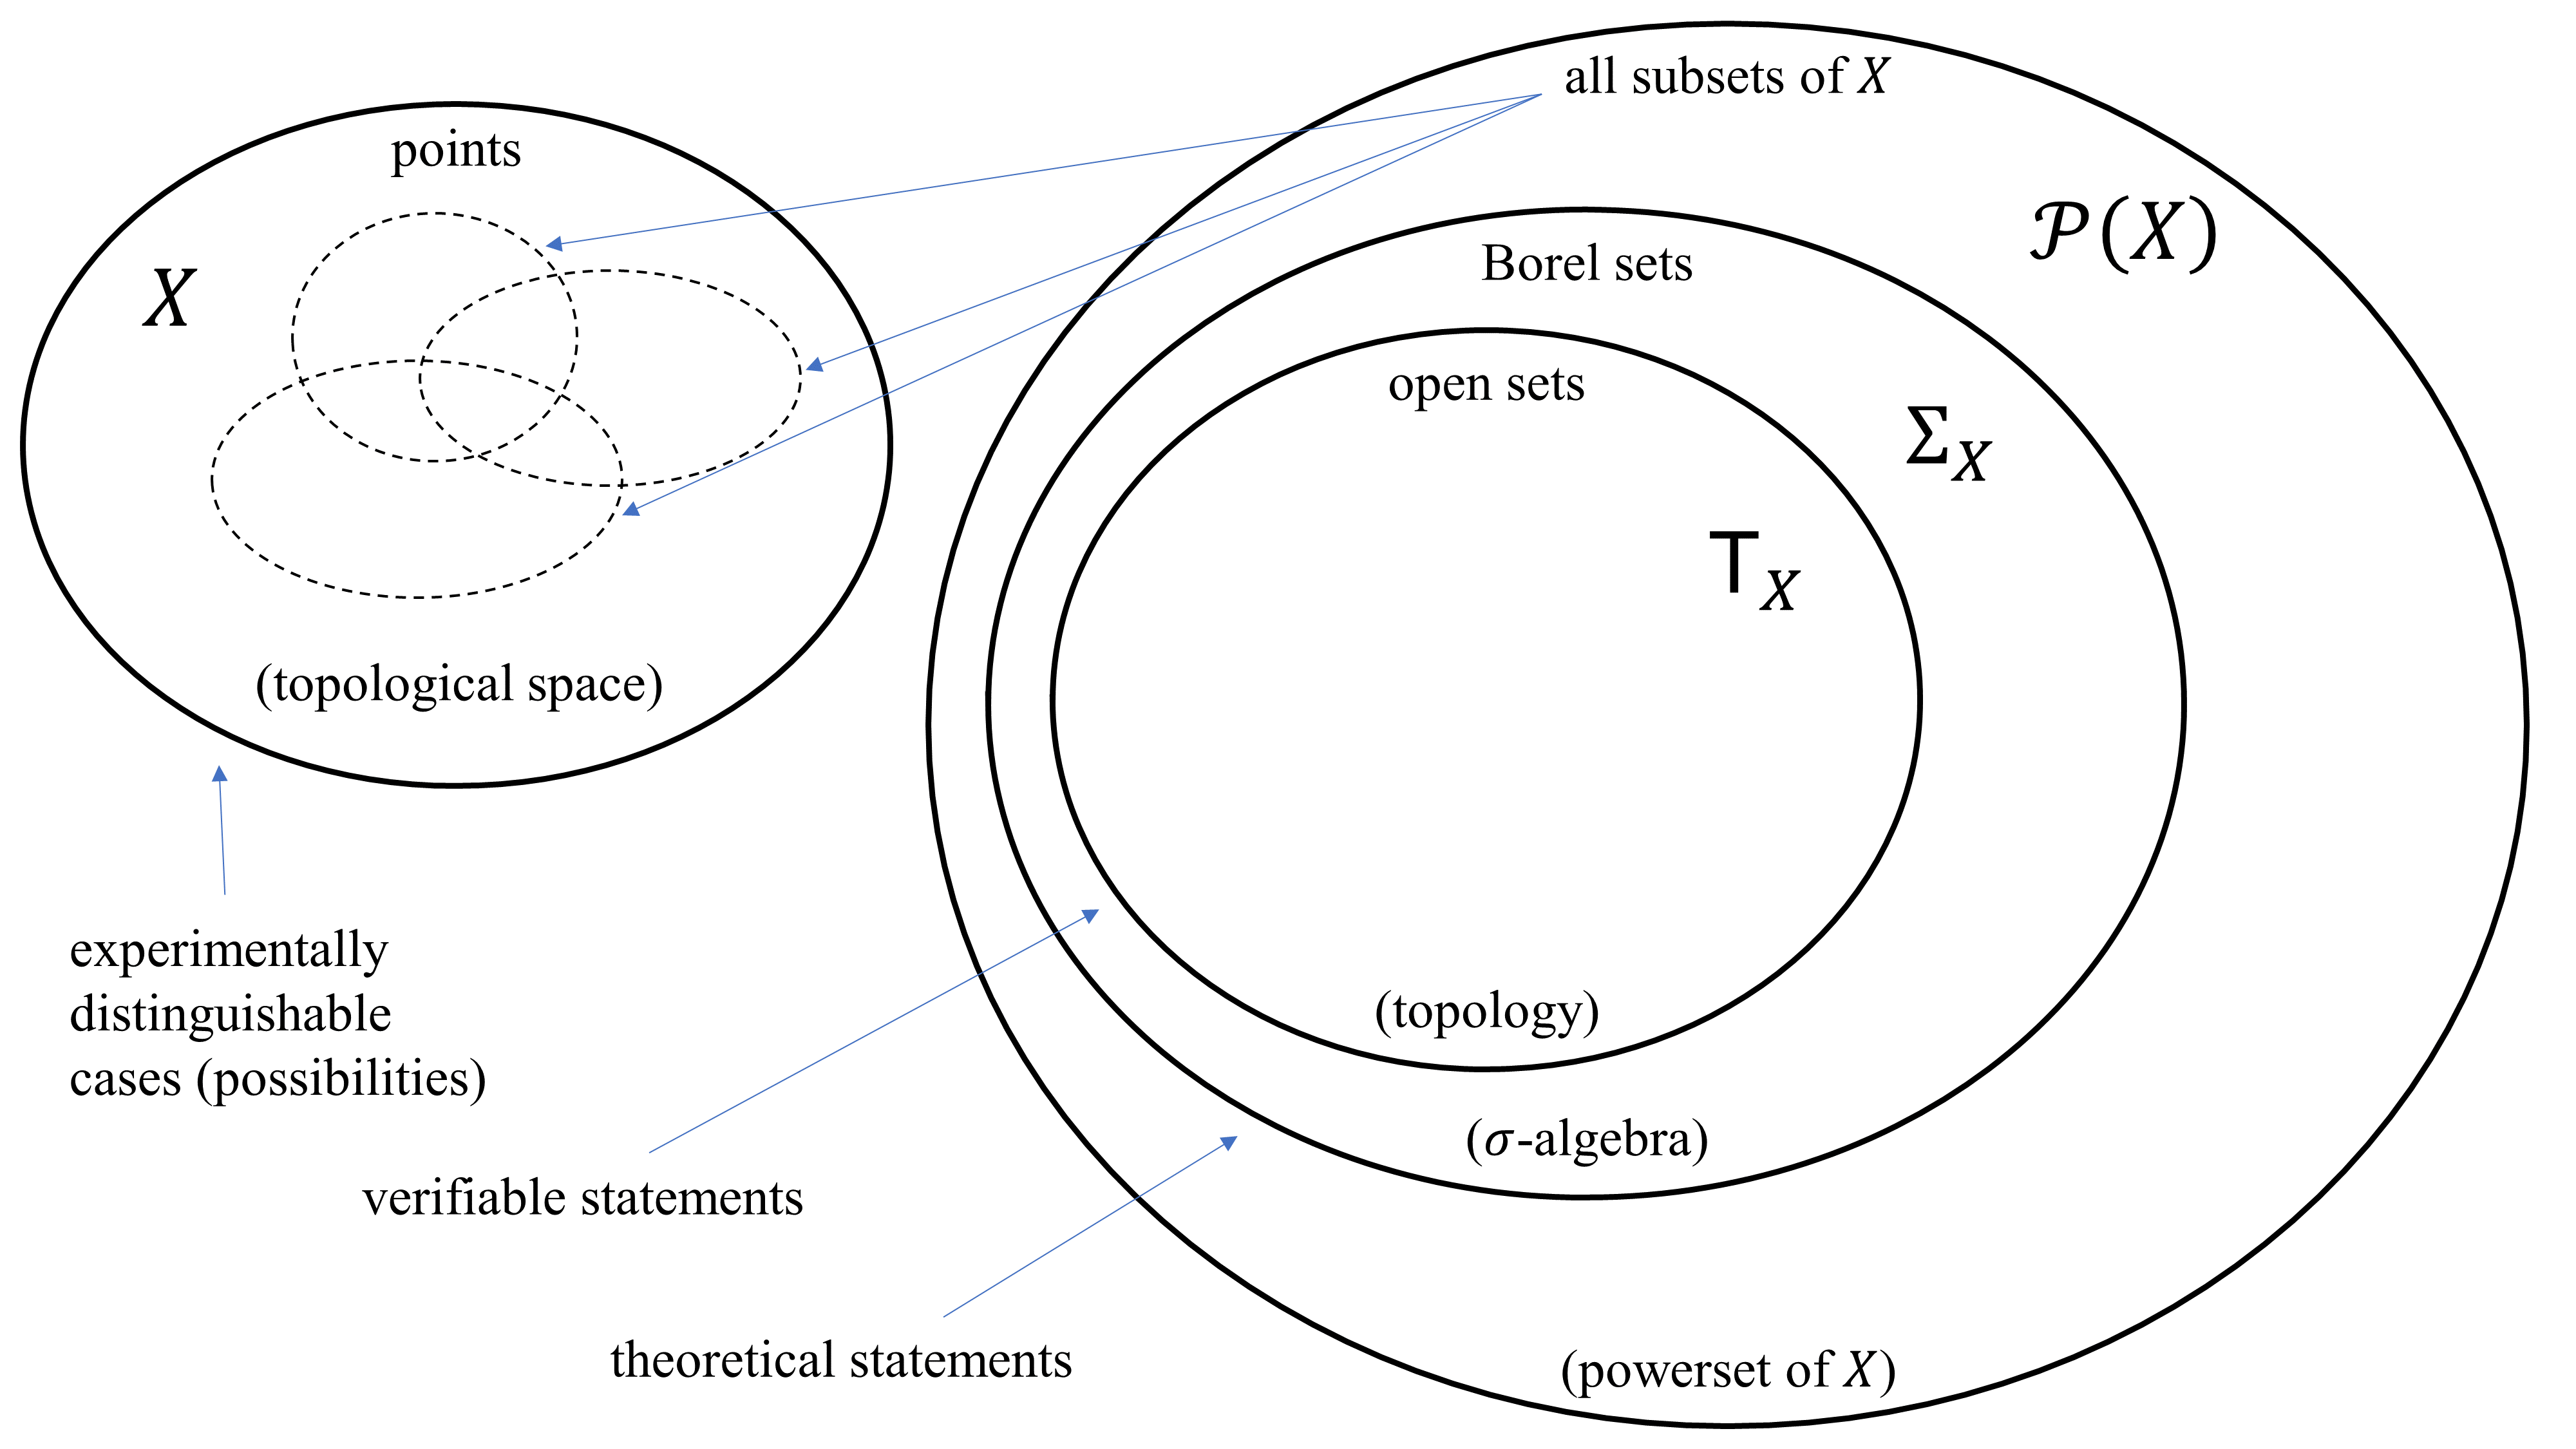
\includegraphics[width=\columnwidth]{Diagram.png}
\end{figure}

The set of points of a topological space represent the possible cases (e.g. all possible values for the mass of a particle). Each element in the topology (i.e. each open set) represents a statement that can be experimentally verified (e.g. the mass of the particle is within a finite precision interval). Each element in the Borel algebra represent a statement that, though it may or may not be experimentally verified, is sound within the theory (e.g. the mass of the particle is exactly zero, the mass of the particle is an irrational number). The Assumptions of Physics framework rederives this structure from the idea that a scientific theory must be logically consistent and evidence based.

\section{Logical context and fundamental axioms}

\section{Experimental and theoretical domains}

\section{Topologies and $\sigma$-algebras}

\section{Experimental relationships and continuous functions}

\bibliography{bibliography}


\end{document}